\documentclass{report}

% ----- useful packages
\usepackage[letterpaper,verbose,pdftex]{geometry}
\usepackage{graphicx} % for including figures
\usepackage{rotating} % for landscape figure
\usepackage{tikz} % for portable graphics
\usepackage[simplified,school]{pgf-umlcd} % for UML class diagrams
\usepackage{amsmath} % align and other math constructs
\usepackage{amssymb} % math symbols
\usepackage{amsthm}
\usepackage{appendix}
\usepackage{listings} % for line-wrapping source code
\usepackage{ulem} % for strike-out font
\usepackage{booktabs} % tables in publication quality
\usepackage{fancyhdr}
\usepackage{fancyvrb,courier} % for more elaborate verbatim envs 
                              % (and bold-face fonts)
\usepackage[parfill]{parskip} % paragraphs begin with empty line rather than indent
\usepackage{setspace} % uncomment below to double-space for editing
\usepackage{url} % for typesetting URL's
%\usepackage[pdftex]{thumbpdf} % for thumbnails in PDF: run thumbpdf perlscript
\usepackage{color}
%\definecolor{mylinkcolor}{rgb}{0,0,0.5}
\usepackage[pdftex, % driver
  hyperfootnotes=false, % if using "footnotes" package
  colorlinks=false, % don't color links
  bookmarks=true,bookmarksnumbered=true, % show numbered bookmarks
  pdfsubject={},pdftitle={},pdfauthor={} % document info
]{hyperref} % more hyperlinks in PDF
%\usepackage{pdfpages} % to include coverpage generated from Word
\usepackage{minitoc}


%% header and footer on every page
\fancypagestyle{plain}{% 
 \fancyhf{} % clear all header and footer fields
% \fancyhead[L]{\small SRI International Proposal \\ ECU 09-445}
 \fancyhead[R]{\leftmark} 
 \fancyfoot[R]{\small \textcopyright\ 2012 SRI International}
 \addtolength{\headheight}{\baselineskip} 
 \renewcommand{\headrulewidth}{0.4pt} 
 \renewcommand{\footrulewidth}{0.4pt}} 
\pagestyle{plain}
\renewcommand{\chaptermark}[1]{\markboth{\thechapter\ #1}{}}

%% AMS LaTeX definitions:
\newtheorem{defi}{Definition}
\newtheorem{lem}{Lemma}

%% customize source code output
\fvset{fontsize=\footnotesize}
\definecolor{keyword}{gray}{0.75}
\lstset{%
basicstyle=\scriptsize\ttfamily,
breaklines=true,
breakindent=0pt,
breakatwhitespace=true,
frame=lines,
fancyvrb=false,
morefvcmdparams=\textcolor 2,
columns=fullflexible,
numbers=left,
numberstyle=\tiny,
keywordstyle=\color{keyword}\bfseries}
\lstloadlanguages{C,[LaTeX]TeX,Java}
\lstdefinestyle{Java}{%
basicstyle=\tiny\ttfamily,numbers=left,numberstyle=\tiny,stepnumber=2,language=Java}
\lstdefinestyle{API}{%
language=Java,numbers=none}
\renewcommand{\lstlistlistingname}{List of Listings} % fit heading with standard ones


% ----- title information
\title{The \LaTeX{} Track Changes System \\ {\large Technical Report}}
\author{%
Linda Briesemeister, Grit Denker, Peter Karp\\
\texttt{firstname.lastname@sri.com}\\
SRI International
}
\date{\today} 

\begin{document}
\maketitle
%{\pagestyle{empty}\cleardoublepage} % uncomment for empty page after title
%\doublespace % uncomment for editing

\dominitoc
\tableofcontents
%\listoftables
%\listoffigures
%\lstlistoflistings

\chapter{Introduction}

	\newcommand{\figscale}{0.6}
\chapter{Content Tracking}
\minitoc

Our change tracking system relies on a version control system underneath that provides us with a database of the history of how each tracked file changes.  We choose the content tracking system called ``git,'' \cite{git} as it matches with important requirements of our system:
\begin{itemize}
\item distributed usage: authors maintain their own repository and efficiently share and merge others, as well as superior offline capabilities
\item available on major platforms %check about Windows!
\item free and open source
\end{itemize}

\section{Traversing History}

\begin{figure}
\centering
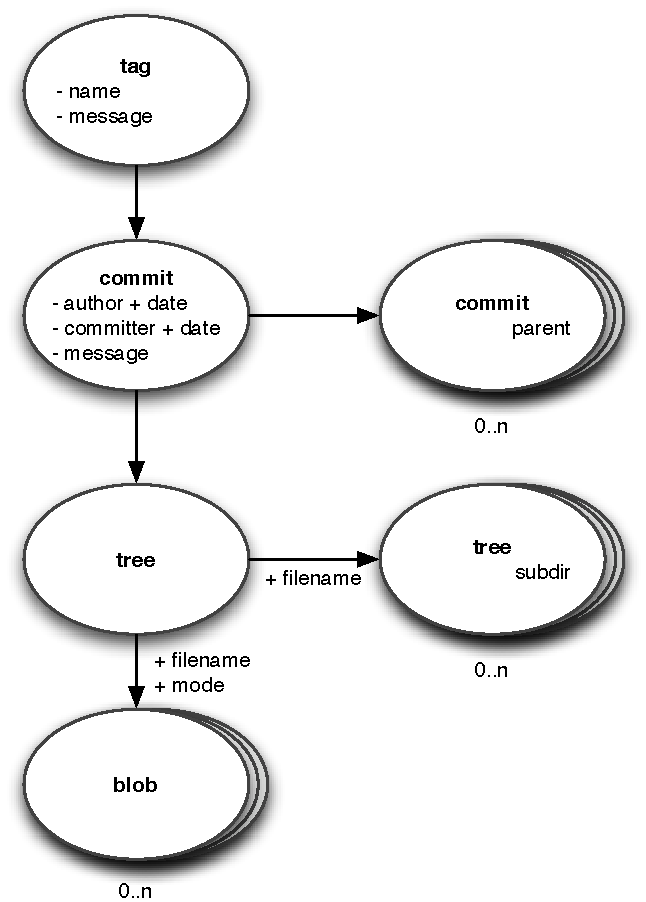
\includegraphics[scale=\figscale]{./figures/git-nodes}
\caption{Node types in Git repositories} \label{fig:git-nodes}
\end{figure}
The anatomy of a git repository is a \textit{directed, acyclic graph} (DAG) with various pointers maintained. There are four types of nodes, which are immutable objects denoted by an SHA-1 hash.  See Figure~\ref{fig:git-nodes} for a graphical representation. 
\begin{enumerate}
\item blob: A leaf node that is the simplest object in git.  Most often it represents a file but can also refer to symbolic links and other artifacts.
\item tree: A tree node encapsulate a directory in git.  It points to blobs and other trees that are subdirectories of this directory.
\item commit: A commit node refers to one tree that represents the state of the files at the time of the commit.  It also refers to other commit nodes that are its parents.  An initial commit has no parents.  A merged commit has more than one parent.
\item tag: A tag node points to one commit.
\end{enumerate}

To obtain the history of a single file in git, we have to traverse the DAG of the commits (more precisely, the tree rooted at the head commit of the currently checked out branch) and search for this individual file in the subtree under each commit.  Figure~\ref{fig:git-commit1} shows an example where a file \texttt{foo.tex} has been modified in a few commits and most notably in the parallel branches.

\begin{figure}
\centering
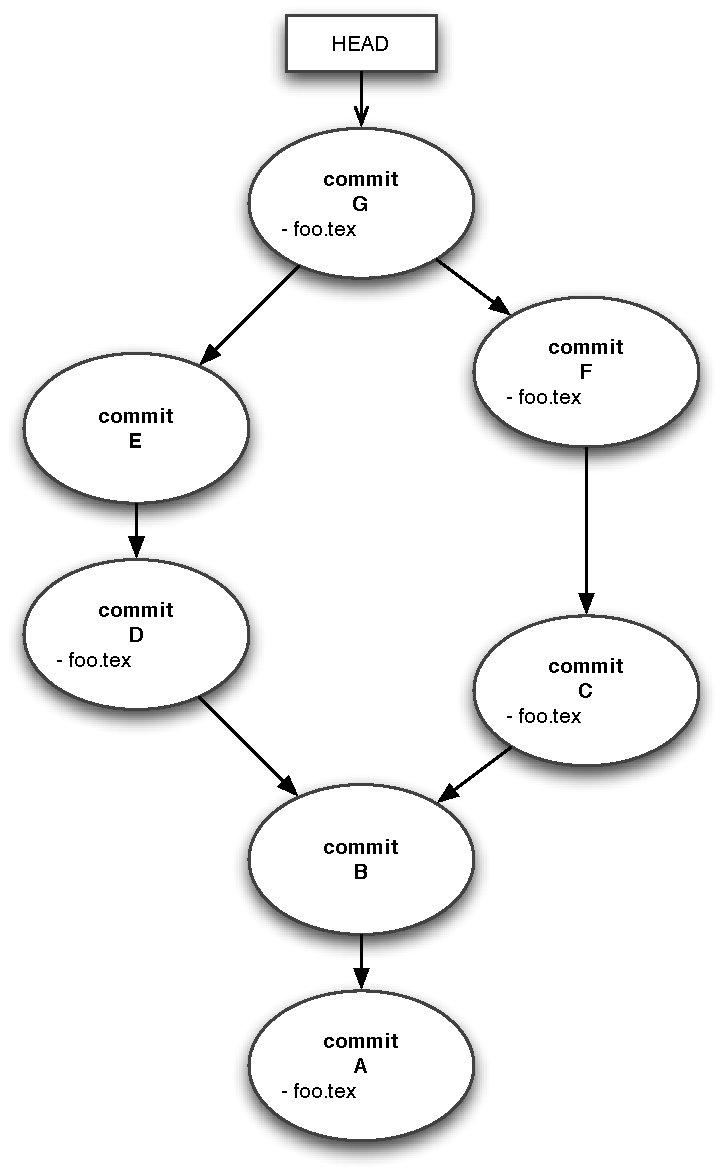
\includegraphics[scale=\figscale]{./figures/git-commit-history1}
\caption{Example commit history for certain file \texttt{foo.tex}} \label{fig:git-commit1}
\end{figure}

As git provides many tools and scripts to deal with the repository, we suggest a two step approach:  First, we obtain the log of the file to identify the commits, in which the contents of the file changed.  Then, we create specialized diffs between each pair of file versions that are adjacent in the history of that file.  Note that the history of the file can be non-linear when branches contain parallel modifications of the file.

\subsection{Commit Graphs}

Here we introduce a few mathematical definitions to be used to clarify the specification of how the change history of a given file is computed.  We assume that the file in question is tracked in a git repository\footnote{We further assume that the git repository currently does not have a detached HEAD reference.}.

\begin{defi}[Commit Graph]
The commit graph $G \subset N \times N$, where $N$ is the set of commit nodes in git, is obtained from traversing the history of commits starting from the HEAD reference until no more nodes can be reached.  The commit graph is directed and acyclic. 
\end{defi}

Most likely, the user's current filter on viewing changes contains a date or revision identifier that will be used to prune the commit graph.

\begin{defi}[Time-Pruned Commit Graph]
We obtain the time-pruned commit graph for a given date as follows.  Traverse the commit graph from the HEAD in a modified breadth-first search (in that nodes can be visited more than once and the resulting graph is not necessarily a tree).  When the given date is later than a commit encountered from traversing the graph, the node is not included in the pruned graph and the search continues at the parent.  Then, all nodes in the resulting graph have time stamps that are later or at the given date.
When the graph is pruned by revision identifier, we follow the same procedure as above with the time stamp of the commit node denoted by the revision identifier.
\end{defi}

\begin{figure}
\centering
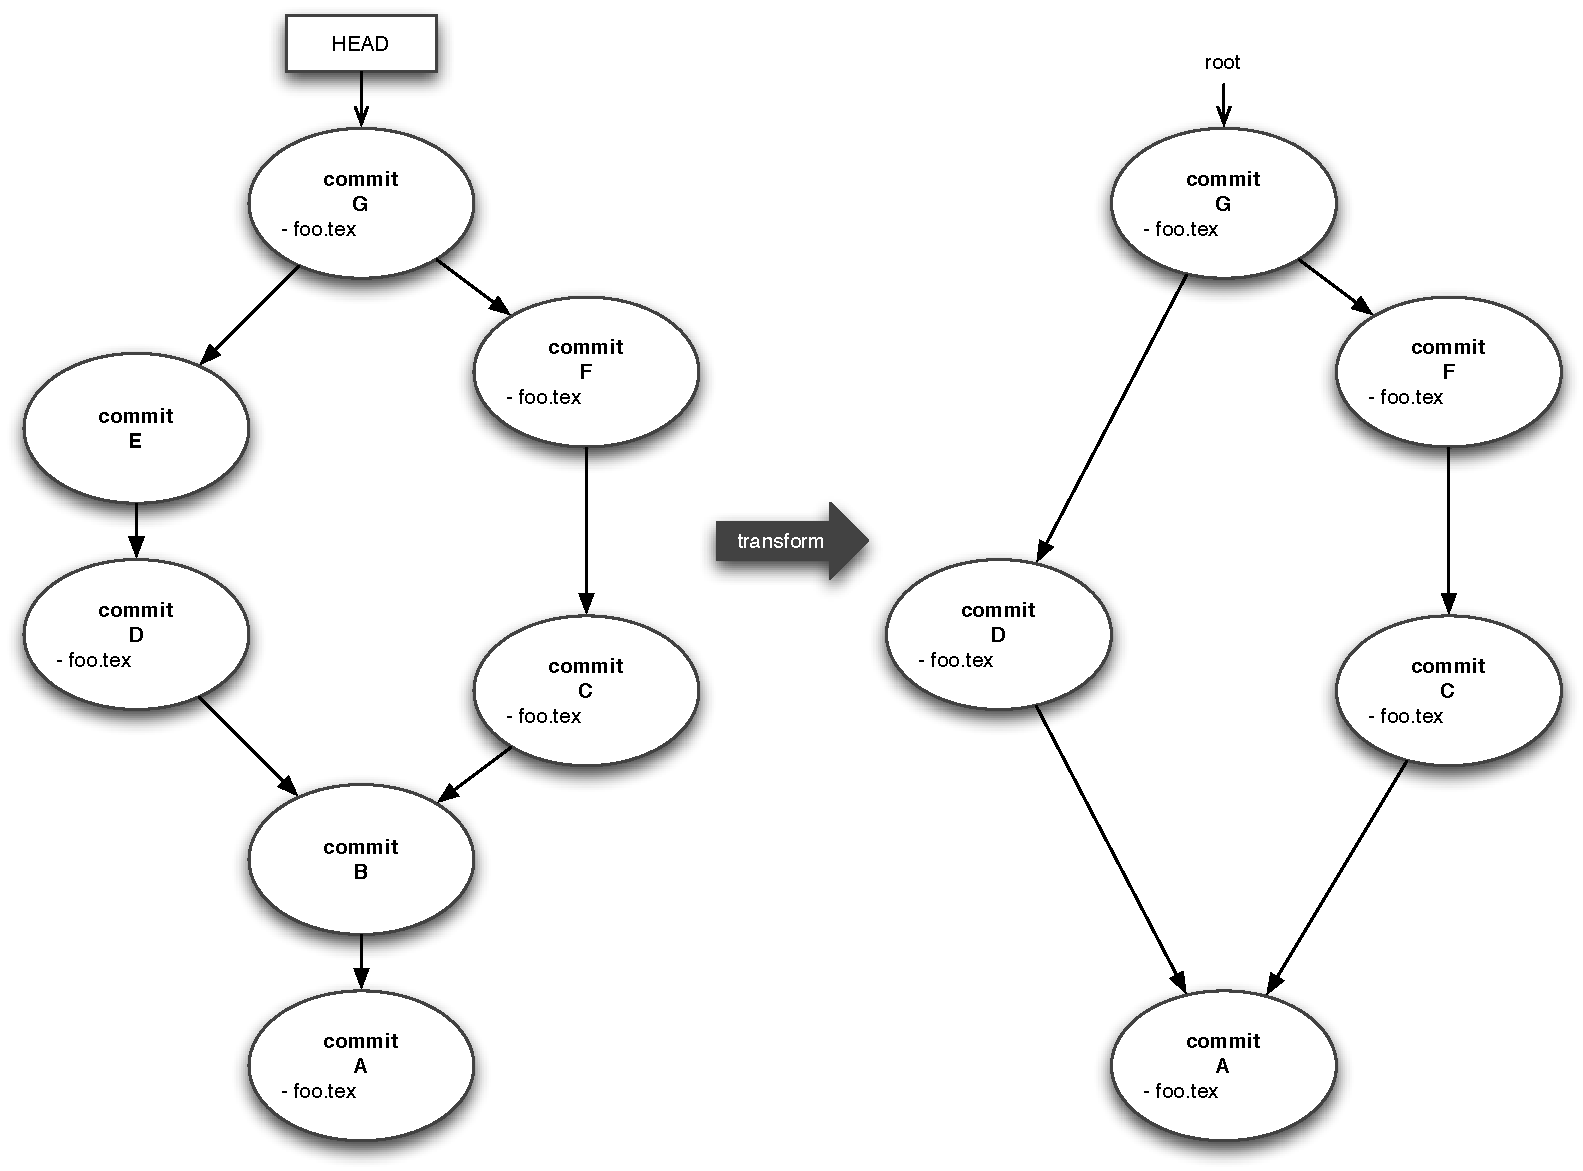
\includegraphics[width=0.9\textwidth]{./figures/git-commit-history2b}
\caption{Transforming commit graph given file \texttt{foo.tex}} \label{fig:git-commit2b}
\end{figure}

Next, we describe how to transform the (potentially time-pruned) commit graph when we obtain the changes of a certain file.  Figure~\ref{fig:git-commit2b} depicts an example of this transformation.

\begin{defi}[File-Specific Commit Graph]
We mark all commit nodes that contain changes to the given file as the set $N^{*} \subseteq N$. Then, we traverse the commit graph again from the HEAD pointer, this time in depth-first search (with the modification of visiting nodes multiple times, as the resulting graph is not necessarily a tree). If the visited node $n_{current}$ is element of $N^{*}$, we include it in the new graph. Keeping track of the last node added (or, if this is the first one, we use the HEAD reference), we add the edge $(n_{last\_added}, n_{current})$ to the new, file-specific commit graph $G^{*}$. If $n_{current}$ is already part of the graph, we backtrack to the next branch to traverse.  When backtracking, the pointer to the last node added has to be adjusted.
\end{defi}

\begin{lem}
The transformed file-specific commit graph is always rooted at exactly one commit node.  If during traversal we encounter a merge commit node with more than one child, and at least two branches under this parent contain changes to the given file, then the merge commit must also contain changes to the said file and thus have the merge commit be included in $G^{*}$.  Therefore, we cannot construct a situation, in which the root pointer would reference more than one commit node in $G^{*}$.
\end{lem}

\begin{figure}
\centering
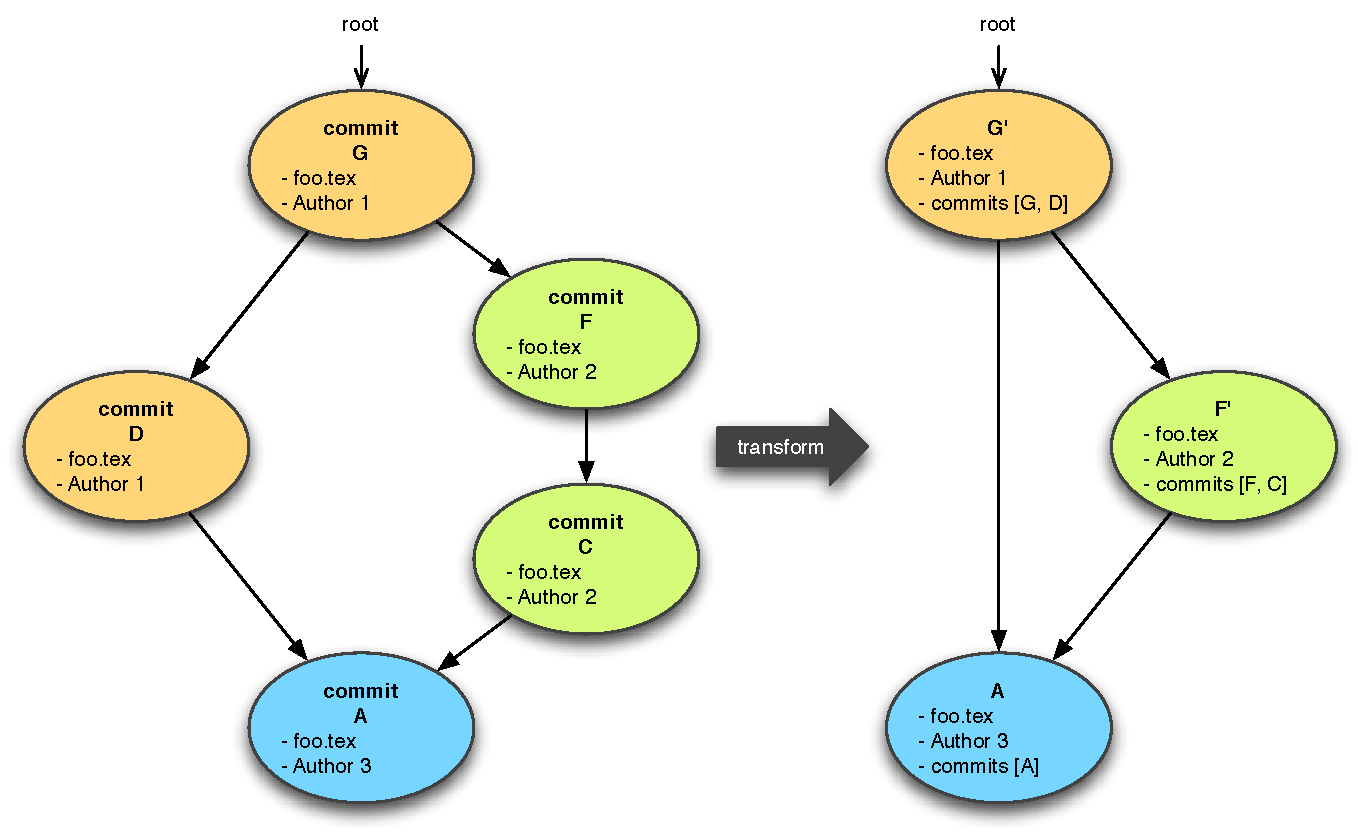
\includegraphics[width=0.9\textwidth]{./figures/git-commit-history3b}
\caption{Subsuming commits of same authors} \label{fig:git-commit3b}
\end{figure}

Finally, we describe how the new commit graph gets further transformed to subsume subsequent edits of the same author. Figure~\ref{fig:git-commit3b} shows such an example transformation.  We decide to only subsume subsequent commits if they are part of a linear commit history in the commit graph.  When the date, time, and revision information of subsumed commits is displayed to the user, there will be ranges as a subsumed commit node now potentially refers to multiple commits from the original graph.

more details and definitions for collapsing commits by same author
%\begin{defi}[Author-Subsumed Commit Graph]
%We traverse a given commit graph again using (a modified) depth-first search.  We take note of the author name in the last commit node visited $s_{last\_author}$.  If the currently visited node has the same author name, we build up a list of references to the original commit node and drop this node
%\end{defi}

%\begin{figure}
%\centering
%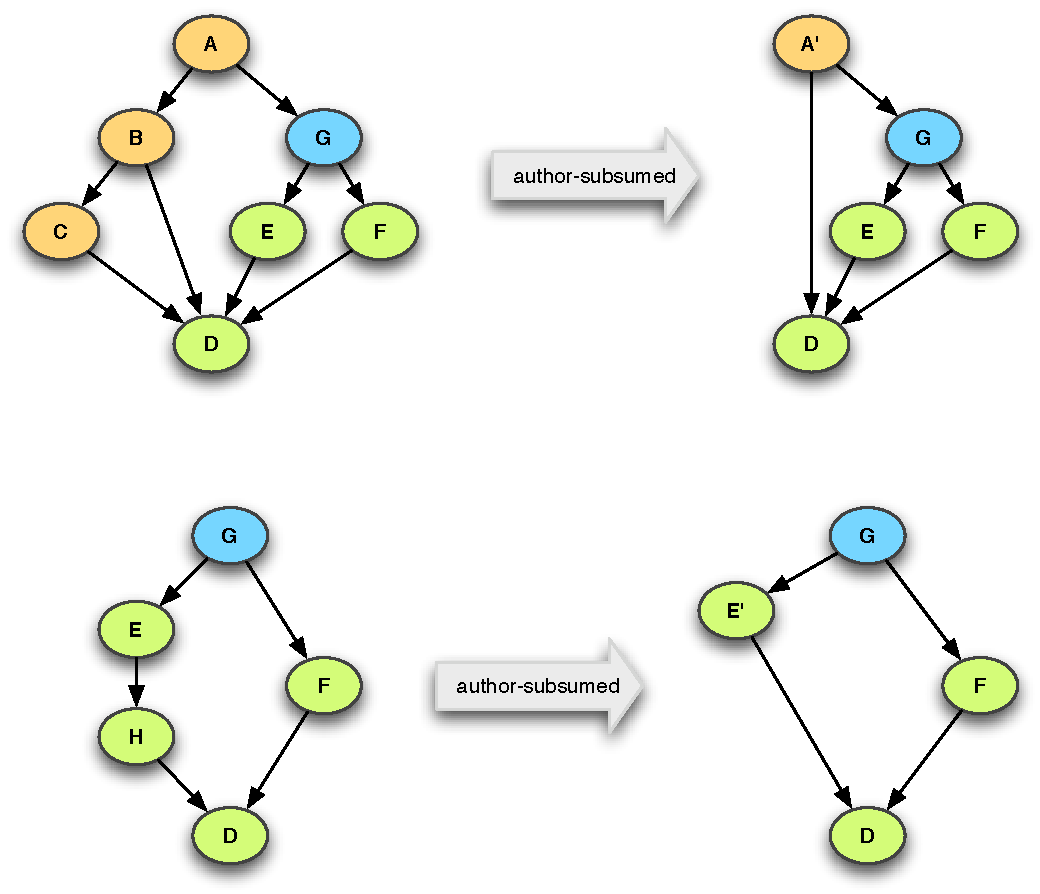
\includegraphics[width=0.9\textwidth]{./figures/tmp-examples}
%\caption{2 examples to discuss} \label{fig:tmp-examples}
%\end{figure}

%Subsume adjacent commits by same author under the latest one?  Makes sense when looking at many commits (we might commit automatically every time the editing author saves when in LTC mode). Also makes sense as LTC is motivated by being interested in other people's changes but not how often or fine-grained the author's commits are.

\section{Serializing Parallel Changes}

%\begin{figure}
%\centering
%%
%\caption{Example of serializing parallel branches for accumulating changes} \label{fig:example-serialization}
%\end{figure}

If we encounter branches in the commit graph, we serialize the parallel changes using the date and time information in the last commit node before the merge commit.  Then, the changes are applied in order of the time stamps.%, as Figure~\ref{fig:example-serialization} depicts.




\section{Filtering}

Filtering the view of changes is the central element to provide real usability of our change tracking capability.  Table~\ref{tab:filter} gives an overview of the choices the user can make to filter the amount of changes displayed.

\begin{table}
\centering
\begin{tabular}{cp{3.5in}p{1.1in}} \toprule
& Description & Default \\\midrule
Authors & If a set of author names is given, limit the view of changes to only those that the respective authors made. To view own changes, include editing author in set. & empty \\
Date/Revision & Specify a time or revisions of how far back to view.  By default, the view extends back to the last commit of the editing author that was before any commit of another author. & last commit until now\\
``Small Changes'' & choose to view changes in words of length $\geq 3$ and Levenshtein distance between words $\leq 3$ & suppress changes \\
%White Space & choose to view changes in white space (unless it affects LaTeX output such as $\geq 2$ consecutive newlines that create a paragraph) & suppress changes \\
Deletions & choose to view deletions & view changes \\
LaTeX Preamble & choose to view changes in LaTeX preamble & view changes \\
LaTeX Markup & choose to view changes in LaTeX markup (commands) & view changes \\
LaTeX Comments & choose to view changes in LaTeX comments & suppress changes \\
\bottomrule
\end{tabular}
\caption{Filtering options} \label{tab:filter}
\end{table}

more details
\chapter{Pairwise Comparison}\label{sec:compare}
\minitoc

\begin{sidewaysfigure}
\centering
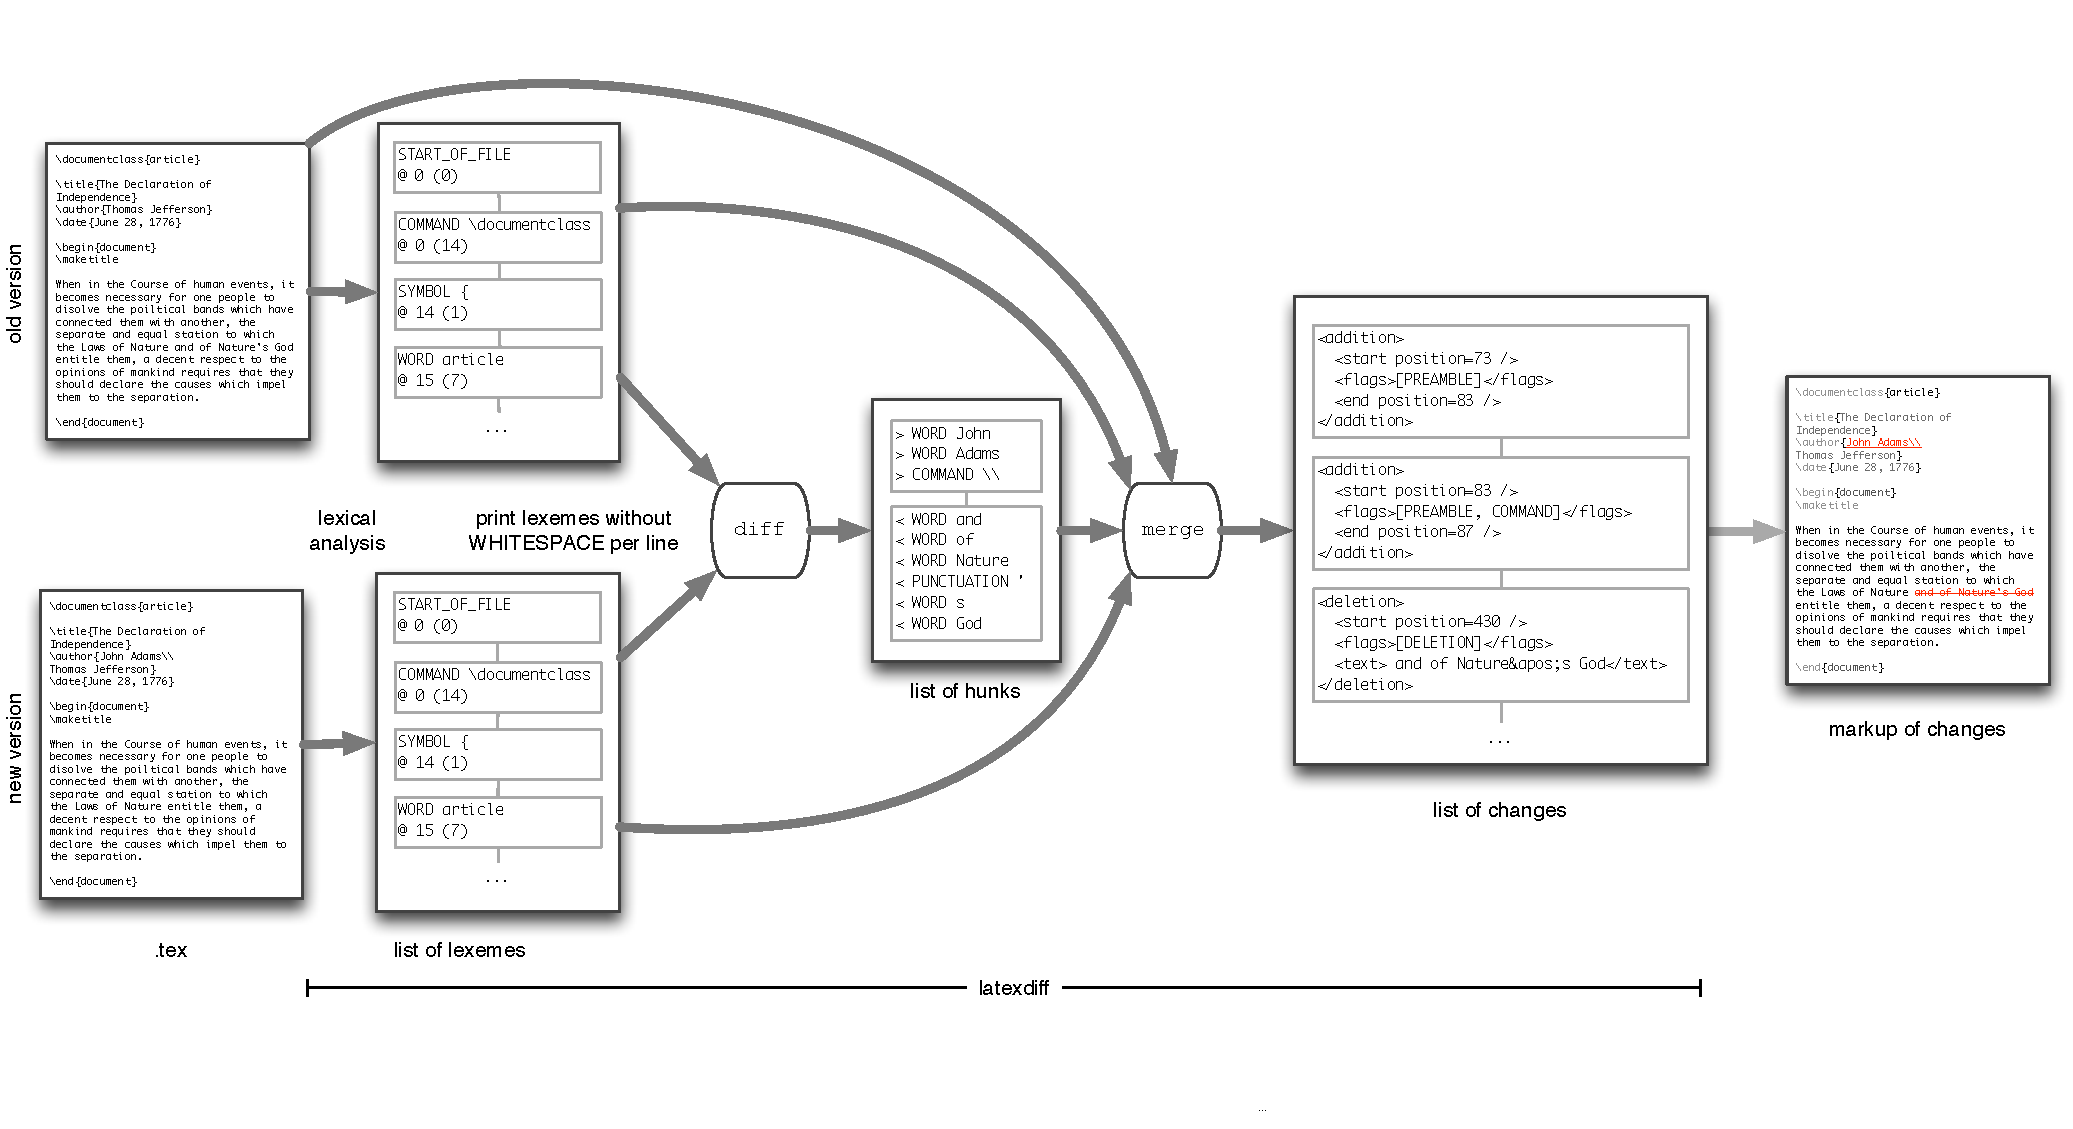
\includegraphics[width=\textwidth]{./figures/latexdiff3}
\caption{Example of performing \texttt{latexdiff} between two versions} \label{fig:latexdiff}
\end{sidewaysfigure}

In this chapter, we describe our LaTeX-aware diff algorithm called \texttt{latexdiff} that compares two LaTeX source files in a meaningful way.  In particular, \texttt{latexdiff} ignores changes in white space unless it creates or removes a paragraph delimiter\footnote{Note that our detection of paragraphs is an approximation: We define paragraph delimiters as two or more newline characters with possibly connecting other white space that occur after the preamble or everywhere in the file if no preamble exists. This definition does not take into account that paragraph space also exists after sectioning commands etc. even if there are less than two newline characters.  It would make our lexical analysis too complicated if we were to parse the LaTeX source files for more accurate detection of paragraph delimiters.} in the body of a LaTeX document. See Figure~\ref{fig:latexdiff} for an overview of \texttt{latexdiff}. 

The output of \texttt{latexdiff} contains additional information on top of the bare differences to aid marking up changes in a file.  For example, we need location information in order to locate changes in the newer version of the file, and flags for filtering certain changes to the viewer.

\section{Lexical Analysis}

Lexical analysis is the process of converting a sequence of characters into a sequence of tokens. Programs performing lexical analysis are called lexical analyzers or lexers.  

\begin{figure} 
\centering
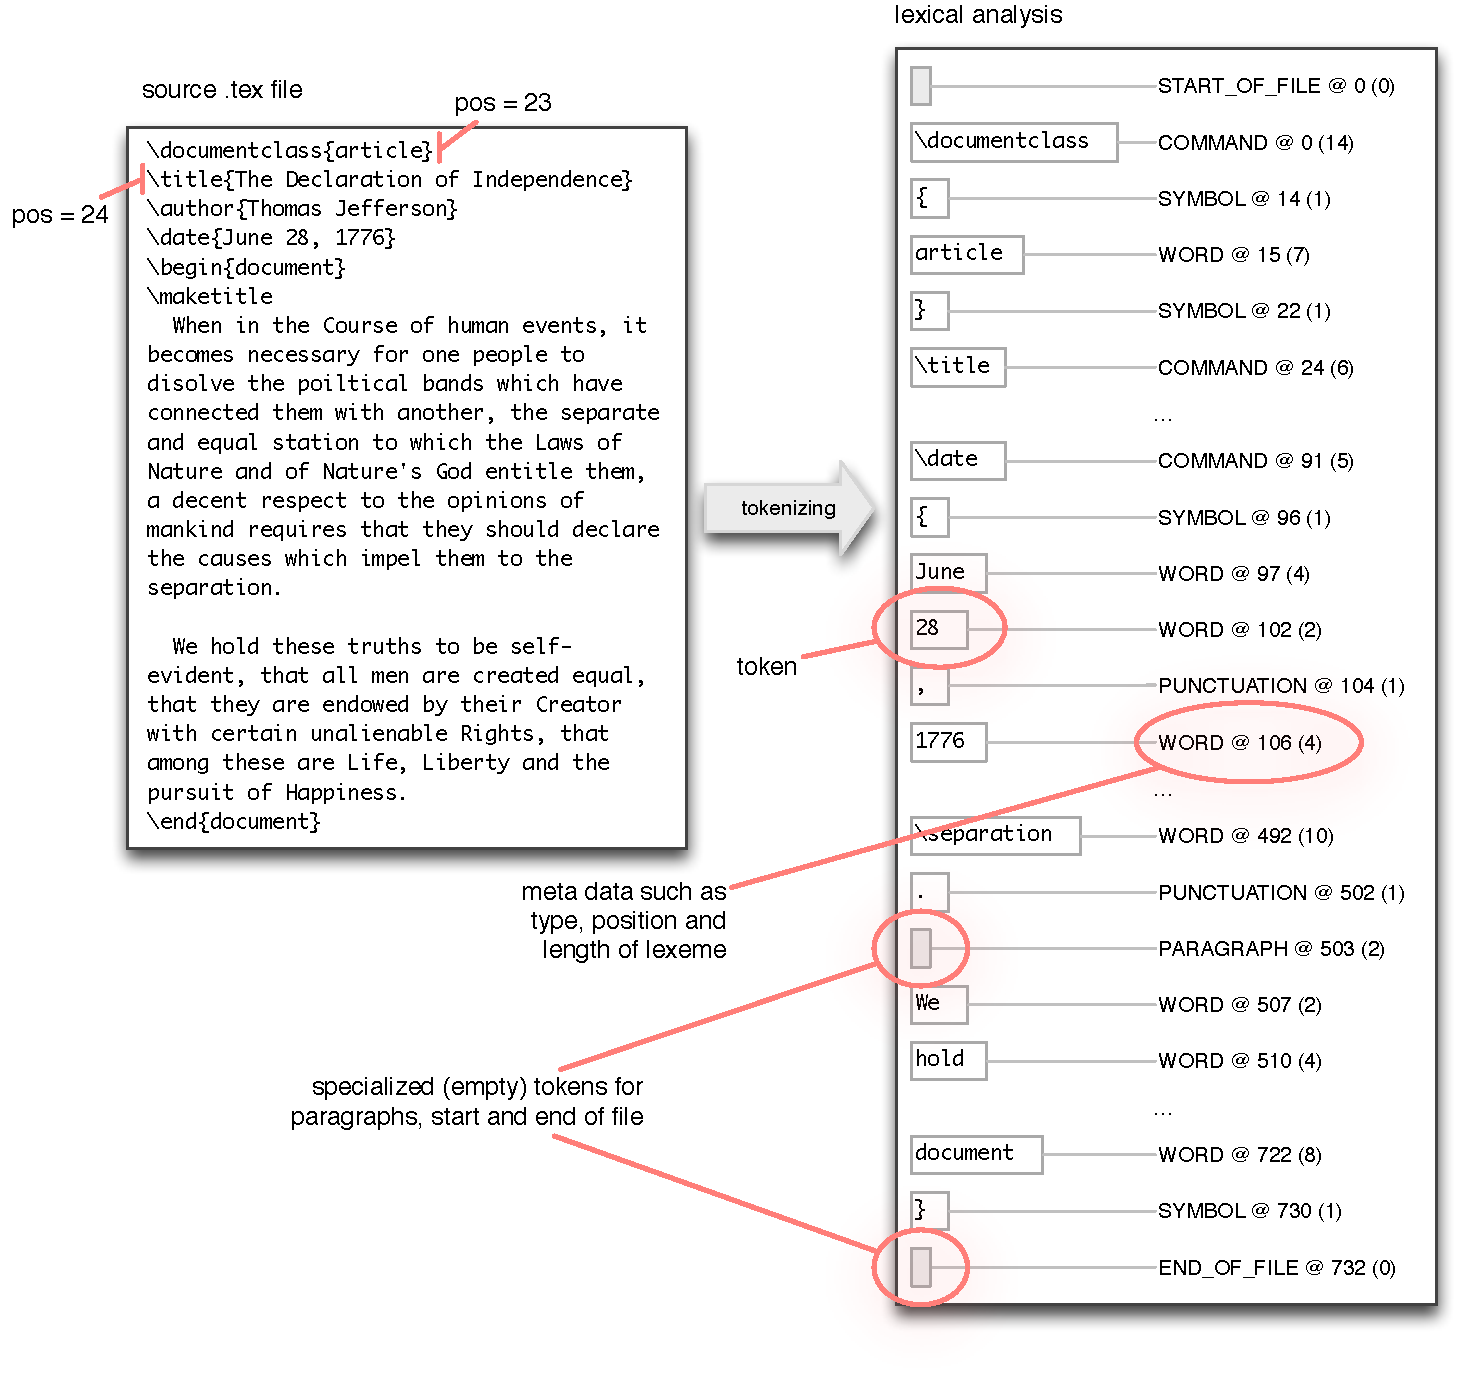
\includegraphics[width=0.9\textwidth]{./figures/tokenizer-example}
\caption{Example of tokenizing source text in preparation for diff'ing} \label{fig:tokenizer-example}
\end{figure}

\lstinputlisting[float,basicstyle=\tiny\ttfamily,
caption={Part of lexer.jflex to perform lexical analysis},label=lst:lexer.jflex,numbers=none,linerange={11-13,22-24,61-130}]{../../../../../ltc-server/src/main/jflex/lexer.jflex}

We call the tokens generated by lexical analysis ``lexemes'' and compare source files lexeme-by-lexeme.  A lexeme is a word, a LaTeX command, punctuation, symbols, non-whitespace parts of comments, or paragraph delimiters (see footnote above about the accuracy of detecting paragraph delimiters).  White space is ignored, however, we still need to keep track of location information in order to display the changes in the latest version of the file.  See Figure~\ref{fig:tokenizer-example} for an example of tokenizing a text file.  Listing~\ref{lst:lexer.jflex} shows our preliminary implementation of the tokenizer using JFlex~\cite{jflex}.

%Listing~\ref{lst:lexeme} shows the data type specification in pseudo code of a lexeme.  
The class diagram below shows the data type for a lexeme.  A lexeme is of a certain, enumerated type.  We also carry the contents of the matched text during lexical analysis in a string.  Finally, we need the linear position of the beginning of the lexeme in the text file, where the first possible position is zero, and---for convenience---the length of the lexeme, which is equal to the length of the contents.
%\begin{lstlisting}[numbers=none,emph={Lexeme,Type,Contents,Pos},emphstyle=\bfseries,caption={Data type of lexemes},label=lst:lexeme]
%Lexeme :
%  Type : Enum of 
%         COMMAND, PREAMBLE, COMMENT, PUNCTUATION, SYMBOL, WORD, PARAGRAPH, WHITESPACE, START_OF_FILE, END_OF_FILE
%  Contents : String
%  Pos : int
%\end{lstlisting}

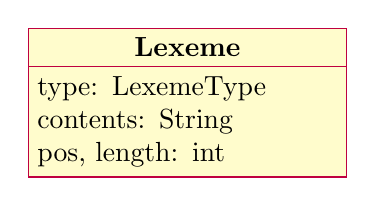
\begin{tikzpicture}
\begin{class}[text width=1.5in]{Lexeme}{0,0}
\attribute{type: LexemeType}
\attribute{contents: String}
\attribute{pos, length: int}
\end{class}
\end{tikzpicture}

\section{Diff'ing the Lexemes}

To prepare the list of lexemes for diff'ing, we first skip WHITESPACE lexemes and then remove PARAGRAPH lexemes from everything in the document preamble (as these are treated as WHITESPACE).  Then, we print each remaining lexeme per line.  The output is the lexeme type followed by a space and the contents for all types except PREAMBLE (matches a constant, therefore irrelevant), PARAGRAPH, START\_OF\_FILE and END\_OF\_FILE as the latter two do not match a character.  Then, we apply the well-known Unix diff algorithm (see for example \url{http://en.wikipedia.org/wiki/Diff}) on a line-by-line basis to determine the longest common subsequences between the two lists of lexemes.

The output of diff is a list of hunks of changes.  Each hunk is marked as \textit{added} (a), \textit{deleted} (d), or \textit{changed} (c).  Each hunk comprises differing lines between the inputs that have the same polarity---either inserted in or removed from the second input.

\section{Merging Diff Results} 

After diff'ing the lists of lexemes, we need to merge the output with the meta data of the lexemes to generate a list of changes that can be easily used for marking up changes.  To illustrate the procedures, we are using example files that are printed in the appendix in Section~\ref{sec:src-files}.  The diff results from comparing the tokenized versions of those files are printed in the appendix in Section~\ref{sec:diff-files}.

We define a hierarchy of data types %(see pseudo code in Listing~\ref{lst:change}) 
to contain the information of changes as seen in the class diagram below.  
%\begin{lstlisting}[numbers=none,emph={Change,LexemesList,Type,Text,StartPos,Offset,Flags},emphstyle=\bfseries,caption={Data type of changes},label=lst:change]
%Change :
%  Type : Subclass of Addition, Deletion, Translocation, SmallAddition, SmallDeletion
%  StartPos : int
%  Flags : boolean
%  Text : String (not Translocation)
%  Offset : int (only Translocation)
%  LexemesList : List of Lexemes (only Addition)
%\end{lstlisting}

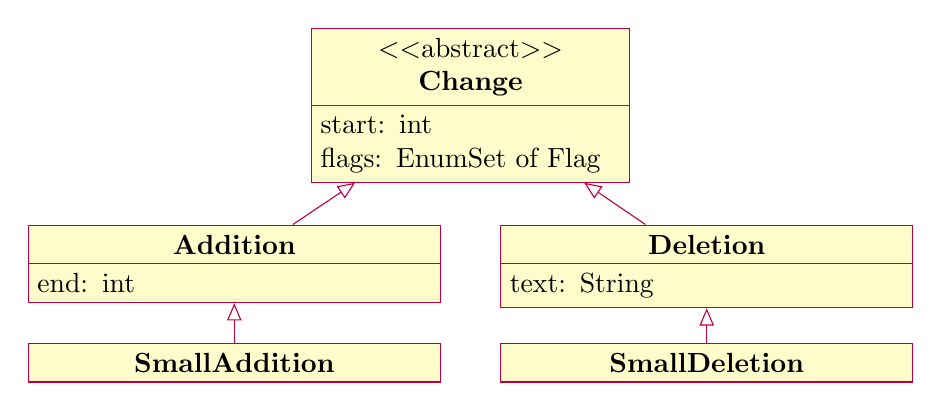
\begin{tikzpicture}
\begin{abstractclass}[text width=1.5in]{Change}{0,0}
\attribute{start: int}
\attribute{flags: EnumSet of Flag}
\end{abstractclass}

\begin{class}{Addition}{-3,-2.5}			
\inherit{Change}
\attribute{end: int}
\end{class}

\begin{class}{Deletion}{3,-2.5}			
\inherit{Change}
\attribute{text: String}
\end{class}

\begin{class}{SmallAddition}{-3,-4}
\inherit{Addition}
\end{class}

\begin{class}{SmallDeletion}{3,-4}
\inherit{Deletion}
\end{class}
\end{tikzpicture}

Each change is a concretization as a subclass of an addition or deletion.  When we detect so-called ``small'' changes, we also use subclasses of addition and deletion to denote these.  Every change contains the linear character position where the change is located in the newer file.  A number of boolean flags facilitate filtering for changes, e.g., those that occur inside LaTeX comments.  Depending on the subclass of the change, there are different additional elements of the data type such as a text field holding the contents of the change (only deletions) or the end position (only additions).

\subsection{Additions and Deletions}

Hunks that are either all inserted or all removed text are handled in a similar manner.  First, we examine the list of consecutive lexemes to identify blocks of COMMENT or COMMAND lexemes.  We split the hunk at these indices such that user filtering becomes easy---if the user does not wish to see changes in comments, the changes that have the respective flag set are easily skipped.

Let us look at the first hunk in the diff output between the first and second version of the example text.  The diff output is merged with meta data information; the first line contains the indices of the change as line numbers into the list of lexemes along with the character denoting the type of change just like the normal diff output.  Then, the lines that differ are preceded by the character showing the polarity of the difference, the lexeme type and possibly contents, then two spaces followed by the meta data of position and length of the lexeme contents.  It is an addition of three lexemes:

\VerbatimInput[frame=lines,label={First hunk of diff output from version 1 to 2},samepage=true,firstline=1,lastline=4]{./examples/diff.1.2.unix}

Our merge algorithm then identifies two sub-hunks; the first consists of two non-comment and non-command lexemes whereas the second one consists of one command lexeme.  The resulting markup information is then split into two additions as can be seen if looking at the XML output corresponding to the same diff hunk:

\VerbatimInput[frame=lines,label={Example of markup information for additions},samepage=true,firstline=1,lastline=10]{./examples/diff.1.2.cml}

When the text editor displays this markup, it looks approximately as follows.

\begin{Verbatim}[frame=lines,label={Markup for first diff block in text editor},samepage=true,showspaces=true,commandchars=+\{\}]
\author+{+textcolor{red}{+underline{John Adams\\}}
\end{Verbatim}

Deletion hunks are processed in a similar way.  Again, the sub-hunks of consecutive COMMENT and COMMAND lexemes are identified.  Looking again at the differences in tokens between the first and second version of the example text, the third hunk of the diff output refers to a deletion.

\VerbatimInput[frame=lines,label={Third hunk of diff output from version 1 to 2},samepage=true,firstline=16,lastline=22]{./examples/diff.1.2.unix}

One difference to handling additions is that we carry the contents of the deletion as a string in order to be able to insert the text when marking up changes.  The resulting chane information in XML format is then:

\VerbatimInput[frame=lines,label={Example of markup information for deletions},samepage=true,firstline=16,lastline=20]{./examples/diff.1.2.cml}

If the user is viewing deletions when in change tracking mode, the editor will look similar to the following:

\begin{Verbatim}[frame=lines,label={Markup of deletion block},numbers=left,firstnumber=12,showspaces=true,commandchars=+\{\}]
separate and equal station to which the Laws of Nature +textcolor{red}{+sout{and of Nature's God }}entitle them,
\end{Verbatim}

\subsection{Replacements and ``Small'' Changes}

If tokens are being replaced (the hunk in diff output is labeled \texttt{c}), we differentiate between small and not small changes.  We compare each lexeme with each other lexeme in the replacement hunk to identify small changes.  As a heuristic of small changes, they are defined as lexemes of the same type and not both space, as well as having a Levenshtein distance of less than 3 and less than the length of the shorter lexeme. In future versions, we may have a better heuristic of detecting small changes. %(THIS MIGHT BE CONFIGURABLE?)

If the change is not small, we label it as a word-level replacement and mark it up as a deletion of the old word and an insertion of the new word.  For an example, look at the difference between version 2 and 3 of the example text file.  The fourth hunk reads as follows.

\VerbatimInput[frame=lines,label={Fourth hunk of diff output from version 2 to 3},samepage=true,firstline=24,lastline=27]{./examples/diff.2.3.unix}

This translates into the following XML code.

\VerbatimInput[frame=lines,label={Example of markup information for replacements},samepage=true,firstline=37,lastline=46]{./examples/diff.2.3.cml}

If the user chose to view deletions, the editor with the marked up replacement may look similar to this:

\begin{Verbatim}[frame=lines,label={Markup of whole word change blocks},numbers=left,firstnumber=12,showspaces=true,commandchars=+\{\}]
becomes+textcolor{blue}{+sout{ imperative}+underline{ necessary }}for
\end{Verbatim}

Now if the change is deemed ``small,'' we need to break down the differences to character level.  For an example, look at the second hunk of diff output between version 2 and 3.

\VerbatimInput[frame=lines,label={Second hunk of diff output from version 2 to 3},samepage=true,firstline=5,lastline=8]{./examples/diff.2.3.unix}

The change hunk above translates into the following markup information in small additions and deletions.  

\VerbatimInput[frame=lines,label={Example of markup information for ``small'' changes},samepage=true,firstline=11,lastline=20]{./examples/diff.2.3.cml}

Now the following shows how small changes may be displayed in an editor.  

\begin{Verbatim}[frame=lines,label={Markup of a small change},samepage=true,showspaces=true,commandchars=+\{\}]
\mak+textcolor{blue}{+sout{t}}e+textcolor{blue}{+underline{t}}itle
\end{Verbatim}

When the hunk denoting a replacement contains more than one line for insertions or deletions, we compare each lexeme of the insertions with each lexeme of the deletions to detect small changes.  Once a direct comparison between two lexemes is considered a small change, we continue the pairwise comparison from the next indices on.  To explain this further, let us look at the fifth hunk of the diff output between version 2 and 3:

\VerbatimInput[frame=lines,label={Fifth hunk of diff output from version 2 to 3},samepage=true,firstline=28,lastline=40]{./examples/diff.2.3.unix}

Here, the first two lexemes of the insertion match with the first two lexemes of the deletion as a small change each.  Then, the third lexeme ``the'' of the insertion is compared with the remaining three lexemes ``ppoilticall,'' ``ties,'' and ``that'' of the deletion but none of these fulfills the requirements of a small change.  As the third lexeme of the deletion constitutes a small change compared to the fourth lexeme of the insertion, we keep the prior lexeme ``the'' as a regular addition for further processing.  The last two lexemes of each also do not match as small changes and are therefore processed as another addition and deletion.

\subsection{Positioning of Changes}

% TODO: add text about tables and overview graphic

\subsubsection{Additions}

\begin{table}
\centering
\begin{tabular}{r@{ or }lll*{3}{c}*{2}{l}} \toprule
\multicolumn{2}{c}{case} & diff & change & $sx_0$ & $sx_1$ & $ex_1$ & start & addition \\
\multicolumn{2}{c}{} & & & $==$ & $==$ & $==$ & & end \\
\multicolumn{2}{c}{} & & & $sy_0$ & $sy_1$ & $ey_1$ & & \\
\midrule
A & C &  
  \difflexemes{C/match//}{C/diff//,D/diff//2mm,F/match//} &
  \changelexemes{C/diff//,D/diff//2mm,F/match//}{C/D/0.08/below} &
 T & T & T & $sx_1 = sy_1$ & $ex_1 = ey_1$ \\
B & D &    
  \difflexemes{B/space/1/,C/match//}{C/diff//,D/diff//2mm,F/match//} &
  \changelexemes{C/diff//,D/diff//2mm,F/match//}{C/D/0.08/below} &
 F & T & T & $sx_1 = sy_1$ & $ex_1 = ey_1$ \\
E & G &  
  \difflexemes{C/match//}{B/space/3/,C/diff//,D/diff//2mm,F/match//} &
  \changelexemes{B/space/3/,C/diff//,D/diff//2mm,F/match//}{B/D/0.08/below} &
 T & F & T & $sx_1$ & $ex_1 = ey_1$ \\
F & H &   
  \difflexemes{B/space/1/,C/match//}{B/space/3/,C/diff//,D/diff//2mm,F/match//} &
  \changelexemes{B/space/3/,C/diff//,D/diff//2mm,F/match//}{B/D/0.08/below} &
 F & F & T & $sx_1$ & $ex_1 = ey_1$ \\
I & K &  
  \difflexemes{C/match//}{C/diff//,D/diff//2mm,E/space/4/,F/match//} &
  \changelexemes{C/diff//,D/diff//2mm,E/space/4/,F/match//}{C/E/0.08/below} &
 T & T & F & $sx_1 = sy_1$ & $ey_1$ \\
J & L &   
  \difflexemes{B/space/1/,C/match//}{C/diff//,D/diff//2mm,E/space/4/,F/match//} &
  \changelexemes{C/diff//,D/diff//2mm,E/space/4/,F/match//}{C/E/0.08/below} &
 F & T & F & $sx_1 = sy_1$ & $ey_1$ \\
M & O & 
  \difflexemes{C/match//}{B/space/3/,C/diff//,D/diff//2mm,E/space/4/,F/match//} &
  \changelexemes{B/space/3/,C/diff//,D/diff//2mm,E/space/4/,F/match//}{B/E/0.08/below} &
 T & F & F & $sx_1$ & $ey_1$ \\
N & P & 
  \difflexemes{B/space/1/,C/match//}{B/space/3/,C/diff//,D/diff//2mm,E/space/4/,F/match//} &
  \changelexemes{B/space/3/,C/diff//,D/diff//2mm,E/space/4/,F/match//}{B/E/0.08/below} &
 F & F & F & $sx_1$ & $ey_1$ \\\midrule
\multicolumn{3}{l}{result} & & & & & $sx_1$ & $ey_1$ \\
\bottomrule
\end{tabular}
\caption{Positioning for additions} \label{tab:pos-additions}
\end{table}

\subsubsection{Deletions}

\begin{table}
\centering
\begin{tabular}{r@{ or }lll*{3}{c}*{3}{l}} \toprule
\multicolumn{2}{c}{case} & diff & change & $sx_0$ & $ex_0$ & $sx_1$ & start & deletion & deletion \\
\multicolumn{2}{c}{} & & & $==$ & $==$ & $==$ & & text & text \\
\multicolumn{2}{c}{} & & & $sy_0$ & $ey_0$ & $sy_1$ & & start & end \\
\midrule
A & I &  
  \difflexemes{C/diff//,D/diff//2mm,F/match//}{C/match//} &  
  \changelexemes{C/diff//,D/diff//2mm,F/match//}{C/D/0.1/above} &
 T & T & T & $sx_1 = sy_1$ & $sx_0 = sy_0$ & $ex_0 = ey_0$  \\
B & J &  
  \difflexemes{B/space/1/,C/diff//,D/diff//2mm,F/match//}{C/match//} &  
  \changelexemes{B/space/1/,C/diff//,D/diff//2mm,F/match//}{B/D/0.1/above} &
 F & T & T & $sx_1 = sy_1$ & $sx_0$ & $ex_0 = ey_0$  \\
C & K & 
  \difflexemes{C/diff//,D/diff//2mm,E/space/2/,F/match//}{C/match//} &  
  \changelexemes{C/diff//,D/diff//2mm,E/space/2/,F/match//}{C/E/0.1/above} &
 T & F & T & $sx_1 = sy_1$ & $sx_0 = sy_0$ & $ey_0$  \\
D & L &  
  \difflexemes{B/space/1/,C/diff//,D/diff//2mm,E/space/2/,F/match//}{C/match//} &  
  \changelexemes{B/space/1/,C/diff//,D/diff//2mm,E/space/2/,F/match//}{B/E/0.1/above} &
 F & F & T & $sx_1 = sy_1$ & $sx_0$ & $ey_0$  \\
E & M & 
  \difflexemes{C/diff//,D/diff//2mm,F/match//}{B/space/3/,C/match//} &  
  \changelexemes{C/diff//,D/diff//2mm,E/space/3/,F/match//}{C/D/0.1/above} &
 T & T & F & $sx_1$ & $sx_0 = sy_0$ & $ex_0 = ey_0$  \\
F & N &  
  \difflexemes{B/space/1/,C/diff//,D/diff//2mm,F/match//}{B/space/3/,C/match//} &  
  \changelexemes{B/space/1/,C/diff//,D/diff//2mm,E/space/3/,F/match//}{B/D/0.1/above} &
 F & T & F & $sx_1$ & $sx_0$ & $ex_0 = ey_0$  \\
G & O &  
  \difflexemes{C/diff//,D/diff//2mm,E/space/2/,F/match//}{B/space/3/,C/match//} &    
  \changelexemes{C/diff//,D/diff//2mm,E/space/3/,F/match//}{C/D/0.1/above} &
 T & F & F & $sx_1$ & $sx_0 = sy_0$ & $ex_0$  \\
H & P & 
  \difflexemes{B/space/1/,C/diff//,D/diff//2mm,E/space/2/,F/match//}{B/space/3/,C/match//} &  
  \changelexemes{B/space/1/,C/diff//,D/diff//2mm,E/space/3/,F/match//}{B/D/0.1/above} &
 F & F & F & $sx_1$ & $sx_0$ & $ex_0$  \\
\midrule
\multicolumn{3}{l}{result} & & & & & $sx_1$ & $sx_0$ & $ex_0$ or $ey_0$ \\
\bottomrule
\end{tabular}
\caption{Positioning for deletions} \label{tab:pos-deletions}
\end{table}

\subsubsection{Replacements}

\begin{table}
\begin{adjustwidth}{-1in}{-1in}\centering  %  make the table centered into the margins
\begin{tabular}{cll*{4}{c}*{4}{l}} \toprule
case & diff & change & $sx_0$ & $ex_0$ & $sx_1$ & $ex_1$ & start & addition & deletion & deletion \\
 & & & $==$ & $==$ & $==$ & $==$ & & end & text & text \\
 & & & $sy_0$ & $ey_0$ & $sy_1$ & $ey_1$ & & & start & end \\
\midrule
A &  
 \difflexemes{C/diff//,D/diff//2mm,F/match//}%
             {C/diff//,D/diff//2mm,F/match//} &
 \changelexemes{C/diff//,D/diff//2mm,F/diff//,G/diff//2mm,I/match//}%
               {C/D/0.1/above,F/G/0.08/below} &
 T & T & T & T & $sx_1 = sy_1$ & $ex_1 = ey_1$ & $sx_0 = sy_0$ & $ex_0 = ey_0$  \\
B &  
 \difflexemes{B/space/1/,C/diff//,D/diff//2mm,F/match//}%
             {C/diff//,D/diff//2mm,F/match//} &
 \changelexemes{B/space/1/,C/diff//,D/diff//2mm,F/diff//,G/diff//2mm,I/match//}%
               {B/D/0.1/above,F/G/0.08/below} &
 F & T & T & T & $sx_1 = sy_1$ & $ex_1 = ey_1$ & $sx_0$ & $ex_0 = ey_0$  \\
C &  
 \difflexemes{C/diff//,D/diff//2mm,E/space/2/,F/match//}%
             {C/diff//,D/diff//2mm,F/match//} &
 \changelexemes{C/diff//,D/diff//2mm,E/space/2/,F/diff//,G/diff//2mm,I/match//}%
               {C/E/0.1/above,F/G/0.08/below} &
 T & F & T & T & $sx_1 = sy_1$ & $ex_1 = ey_1$ & $sx_0 = sy_0$ & $ey_0$  \\
D &  
 \difflexemes{B/space/1/,C/diff//,D/diff//2mm,E/space/2/,F/match//}%
             {C/diff//,D/diff//2mm,F/match//} &
 \changelexemes{B/space/1/,C/diff//,D/diff//2mm,E/space/2/,F/diff//,G/diff//2mm,I/match//}%
               {B/E/0.1/above,F/G/0.08/below} &
 F & F & T & T & $sx_1 = sy_1$ & $ex_1 = ey_1$ & $sx_0$ & $ey_0$  \\
E &  
 \difflexemes{C/diff//,D/diff//2mm,F/match//}%
             {B/space/3/,C/diff//,D/diff//2mm,F/match//} &
 \changelexemes{C/diff//,D/diff//2mm,E/space/3/,F/diff//,G/diff//2mm,I/match//}%
               {C/D/0.1/above,E/G/0.08/below} &
 T & T & F & T & $sx_1$ & $ex_1 = ey_1$ & $sx_0 = sy_0$ & $ex_0 = ey_0$  \\
F &  
 \difflexemes{B/space/1/,C/diff//,D/diff//2mm,F/match//}%
             {B/space/3/,C/diff//,D/diff//2mm,F/match//} &
 \changelexemes{B/space/1/,C/diff//,D/diff//2mm,E/space/3/,F/diff//,G/diff//2mm,I/match//}%
               {B/D/0.1/above,E/G/0.08/below} &
 F & T & F & T & $sx_1$ & $ex_1 = ey_1$ & $sx_0$ & $ex_0 = ey_0$  \\
G &  
 \difflexemes{C/diff//,D/diff//2mm,E/space/2/,F/match//}%
             {B/space/3/,C/diff//,D/diff//2mm,F/match//} &
 \changelexemes{C/diff//,D/diff//2mm,E/space/3/,F/diff//,G/diff//2mm,I/match//}%
               {C/D/0.1/above,E/G/0.08/below} &
 T & F & F & T & $sx_1$ & $ex_1 = ey_1$ & $sx_0 = sy_0$ & $ex_0$  \\
H &  
 \difflexemes{B/space/1/,C/diff//,D/diff//2mm,E/space/2/,F/match//}%
             {B/space/3/,C/diff//,D/diff//2mm,F/match//} &
 \changelexemes{B/space/1/,C/diff//,D/diff//2mm,E/space/3/,F/diff//,G/diff//2mm,I/match//}%
               {B/D/0.1/above,E/G/0.08/below} &
 F & F & F & T & $sx_1$ & $ex_1 = ey_1$ & $sx_0$ & $ex_0$  \\
I &  
 \difflexemes{C/diff//,D/diff//2mm,F/match//}%
             {C/diff//,D/diff//2mm,E/space/4/,F/match//} &
 \changelexemes{C/diff//,D/diff//2mm,F/diff//,G/diff//2mm,H/space/4/,I/match//}%
               {C/D/0.1/above,F/H/0.08/below} &
 T & T & T & F & $sx_1 = sy_1$ & $ey_1$ & $sx_0 = sy_0$ & $ex_0 = ey_0$  \\
J &  
 \difflexemes{B/space/1/,C/diff//,D/diff//2mm,F/match//}%
             {C/diff//,D/diff//2mm,E/space/4/,F/match//} &
 \changelexemes{B/space/1/,C/diff//,D/diff//2mm,F/diff//,G/diff//2mm,H/space/4/,I/match//}%
               {B/D/0.1/above,F/H/0.08/below} &
 F & T & T & F & $sx_1 = sy_1$ & $ey_1$ & $sx_0$ & $ex_0 = ey_0$  \\
K &  
 \difflexemes{C/diff//,D/diff//2mm,E/space/2/,F/match//}%
             {C/diff//,D/diff//2mm,E/space/4/,F/match//} &
 \changelexemes{C/diff//,D/diff//2mm,E/space/2/,F/diff//,G/diff//2mm,H/space/4/,I/match//}%
               {C/E/0.1/above,F/H/0.08/below} &
 T & F & T & F & $sx_1 = sy_1$ & $ey_1$ & $sx_0 = sy_0$ & $ey_0$  \\
L &  
 \difflexemes{B/space/1/,C/diff//,D/diff//2mm,E/space/2/,F/match//}%
             {C/diff//,D/diff//2mm,E/space/4/,F/match//} &
 \changelexemes{B/space/1/,C/diff//,D/diff//2mm,E/space/2/,F/diff//,G/diff//2mm,H/space/4/,I/match//}%
               {B/E/0.1/above,F/H/0.08/below} &
 F & F & T & F & $sx_1 = sy_1$ & $ey_1$ & $sx_0$ & $ey_0$  \\
M &  
 \difflexemes{C/diff//,D/diff//2mm,F/match//}%
             {B/space/3/,C/diff//,D/diff//2mm,E/space/4/,F/match//} &
 \changelexemes{C/diff//,D/diff//2mm,E/space/3/,F/diff//,G/diff//2mm,H/space/4/,I/match//}%
               {C/D/0.1/above,E/H/0.08/below} &
 T & T & F & F & $sx_1$ & $ey_1$ & $sx_0 = sy_0$ & $ex_0 = ey_0$  \\
N &  
 \difflexemes{B/space/1/,C/diff//,D/diff//2mm,F/match//}%
             {B/space/3/,C/diff//,D/diff//2mm,E/space/4/,F/match//} &
 \changelexemes{B/space/1/,C/diff//,D/diff//2mm,E/space/3/,F/diff//,G/diff//2mm,H/space/4/,I/match//}%
               {B/D/0.1/above,E/H/0.08/below} &
 F & T & F & F & $sx_1$ & $ey_1$ & $sx_0$ & $ex_0 = ey_0$  \\
O &  
 \difflexemes{C/diff//,D/diff//2mm,E/space/2/,F/match//}%
             {B/space/3/,C/diff//,D/diff//2mm,E/space/4/,F/match//} &
 \changelexemes{C/diff//,D/diff//2mm,E/space/3/,F/diff//,G/diff//2mm,H/space/4/,I/match//}%
               {C/D/0.1/above,E/H/0.08/below} &
 T & F & F & F & $sx_1$ & $ey_1$ & $sx_0 = sy_0$ & $ex_0$  \\
P &  
 \difflexemes{B/space/1/,C/diff//,D/diff//2mm,E/space/2/,F/match//}%
             {B/space/3/,C/diff//,D/diff//2mm,E/space/4/,F/match//} &
 \changelexemes{B/space/1/,C/diff//,D/diff//2mm,E/space/3/,F/diff//,G/diff//2mm,H/space/4/,I/match//}%
               {B/D/0.1/above,E/H/0.08/below} &
 F & F & F & F & $sx_1$ & $ey_1$ & $sx_0$ & $ex_0$  \\
\midrule
\multicolumn{3}{l}{result} & & & & & $sx_1$ & $ey_1$ & $sx_0$ & $ex_0$ or $ey_0$ \\
\bottomrule
\end{tabular}
\caption{Positioning for replacements} \label{tab:pos-replacements}
\end{adjustwidth}
\end{table}

\subsection{Implementation in Java}

Listing~\ref{lst:merge} contains a reference implementation in Java and provides more details of the merge function.

The function call receives the linked list of hunks from the prior diff operation as well as the two lists of lexemes, which were the input to diff (modified as pairs of type and contents) as parameters.  The function has also access to global variables containing the source of the texts that are being compared.  

The outer for-loop starting in line 174 iterates through the linked list of change hunks that the diff operation produced.

In line 182, we examine hunks that are replacements for containing small changes.  There, we need to compare each lexeme of the deletion with each lexeme of the insertion until we find a matching small change.  In that case, we continue the pairwise comparison of lexemes with the indices that are greater than the small change.  In variable \texttt{newHunks} we collect the indices and lengths of new hunks that are created when pairs of lexemes denote a small change in the current hunk being processed.  If such small changes exist in the hunk and the hunk does not consist solely of small changes, we link these new hunks back into the chain of processed hunks for normal additions and deletions in lines 260--294.

Starting with line 260 and 275, we handle normal additions and deletions, respectively.  Calling the function \texttt{getIndices} provides a list of index pairs that may break up the consecutive insertion or deletion of lexemes into chunks that contain only comments, commands, or neither of those.

\lstinputlisting[style=Java,firstnumber=168,caption={Java reference implementation of merge function},label=lst:merge,linerange={167-298}]{../../../../../ltc-server/src/main/java/com/sri/ltc/latexdiff/LatexDiff.java}


\chapter{The Accumulate() Algorithm}

\chapter{Application Programmin Interface (API)}

% ----- references 
%
\bibliographystyle{plain} 
\bibliography{./ltc}
\addcontentsline{toc}{chapter}{Bibliography} 

% ----- appendix
%
\appendix

\chapter{Examples for \texttt{latexdiff}}

In this chapter, we print the contents of example files and the associated \texttt{latexdiff} output.

\section{Source \texttt{.tex} files} \label{sec:src-files}

Thomas Jefferson commits the first version of the document.
\lstinputlisting[language={[LaTeX]TeX},caption={Version 1}]{./examples/independence-version1.tex}

John Adams edits and commits the second version.  He adds himself as an author and adds and deletes two text fragments in the main paragraph.
\lstinputlisting[language={[LaTeX]TeX},caption={Version 2}]{./examples/independence-version2.tex}

Benjamin Franklin edits and commits the third version.  He also adds himself as an author.  His changes include a word replacement, correction of three small typographical errors, as well as adding a new sentence at the end.
\lstinputlisting[language={[LaTeX]TeX},caption={Version 3}]{./examples/independence-version3.tex}

Thomas Jefferson resumes editing in the fourth version.  He reverts a prior change, which results in an addition of a fragment.  He also invokes automatic re-formatting in his text editor, which wraps all lines in 70 characters or less, so that line numbers change.
\lstinputlisting[language={[LaTeX]TeX},caption={Version 4}]{./examples/independence-version4.tex}

\lstinputlisting[language={[LaTeX]TeX},caption={Version 5}]{./examples/independence-version5.tex}

\lstinputlisting[language={[LaTeX]TeX},caption={Version 6}]{./examples/independence-version6.tex}

\section{Tokenizing and Diff'ing} \label{sec:diff-files}

The following diff outputs are obtained using the JFlex analyzer from Listing~\ref{lst:lexer.jflex}.  To run just the lexical analysis on one file:
\begin{Verbatim}[commandchars=+\{\}]
$> java -cp $LTC/LTC-+version.jar com.sri.latexdiff.Lexer <FILE>
\end{Verbatim}

To perform \texttt{latexdiff} between two files, run with:
\begin{Verbatim}[commandchars=+\{\}]
$> java -cp $LTC/LTC-+version.jar com.sri.latexdiff.LatexDiff <FILE1> <FILE2>
\end{Verbatim}

\VerbatimInput[frame=lines,label={Differences between lexical analyses of version 1 and 2}]{./examples/diff.1.2.unix}

\VerbatimInput[frame=lines,label={Differences between lexical analyses of version 2 and 3}]{./examples/diff.2.3.unix}

\VerbatimInput[frame=lines,label={Differences between lexical analyses of version 3 and 4}]{./examples/diff.3.4.unix}

\VerbatimInput[frame=lines,label={Differences between lexical analyses of version 4 and 5}]{./examples/diff.4.5.unix}

\VerbatimInput[frame=lines,label={Differences between lexical analyses of version 5 and 6}]{./examples/diff.5.6.unix}

\section{XML Output} \label{sec:examples-cml}

The following outputs are generated using XML output of the diff'ing algorithm.

\VerbatimInput[frame=lines,label={XML of diff'ing version 1 and 2}]{./examples/diff.1.2.cml}

\VerbatimInput[frame=lines,label={XML of diff'ing version 2 and 3}]{./examples/diff.2.3.cml}

\VerbatimInput[frame=lines,label={XML of diff'ing version 3 and 4}]{./examples/diff.3.4.cml}

\VerbatimInput[frame=lines,label={XML of diff'ing version 4 and 5}]{./examples/diff.4.5.cml}

\VerbatimInput[frame=lines,label={XML of diff'ing version 5 and 6}]{./examples/diff.5.6.cml}
% example files

\end{document}     